\documentclass{beamer}
\usepackage[utf8]{inputenc}
\usepackage[english]{babel}
\setbeamersize{text margin left=10pt, text margin right=10pt} %new code
\usepackage{graphicx}
\usepackage{float}
\usepackage{animate}
\usepackage{movie15}
\usepackage{breqn}
\usepackage{tcolorbox, amsmath}
\usepackage{subcaption}
\newcommand{\mysetminus}{\mathbin{\fgebackslash}}

\setbeamerfont{headline}{size=\small}


%----------------------------------------------------------------------------------------
%	 Package
%----------------------------------------------------------------------------------------
\usepackage{color}
\usepackage{url}
\usepackage{minted}		% listing code
\beamertemplatenavigationsymbolsempty

\definecolor{cadmiumred}{rgb}{0.8, 0.8, 0.8}

%----------------------------------------------------------------------------------------
%	 Presentation settings
%----------------------------------------------------------------------------------------

\usetheme{CambridgeUS}
\usecolortheme{beaver}


\setbeamertemplate{itemize items}[triangle] 
\setbeamertemplate{enumerate items}[default]
 
\title[Bigram Anchor Words Topic Model]{{\normalsize ANALYSIS OF IMAGES SOCIAL NETWORKS AND TEXTS}\\
	\vspace{1cm}
	\textbf{\textcolor{black}{Bigram Anchor Words Topic Model}}}

\author{Ashuha Arseniy, Loukachevitch Natalia}
\institute[]{
	Moscow Institute of Physics and Technology
	
	Research Computing Center of Lomonosov Moscow State University
	
	\medskip
	
	\href{mailto:ars.ashuha@gmail.com}{\nolinkurl{ars.ashuha@gmail.com}} 
	\href{mailto:louk\_nat@mail.ru}{\nolinkurl{louk\_nat@mail.ru}}}


\date{April 29, 2016}

\newcommand{\Expect}{\mathsf{E}}
\newcommand{\MExpect}{\mathsf{M}}
\newcommand{\cov}{\mathsf{cov}}


\begin{document}
%----------------------------------------------------------------------------------------
%	 Title
%----------------------------------------------------------------------------------------
\begin{frame}
	\titlepage 
\end{frame}

\section*{Topic modeling}

\subsection*{Basic}
\begin{frame}
	  
	\textcolor{red}{Motivation}
	\begin{itemize}
	   \item Nowadays we have a lot of data, but usually \textbf{it is unlabled}
	   \item We wont to extract structure from document collection \textbf{unsupervised}
	\end{itemize}
	
	\vspace{0.2cm}
	  
	\textcolor{red}{Haw can we get this goal?}
	\begin{itemize}
		   \item Topic modeling is a powerful tool for document collection analysis
		  \item Unformally, topic is a semantically related set of words
		
		\vspace{0.1cm}
		  \hspace{0.2cm} \textcolor{gray}{sample}: \textit{geom rna fast dna sequence alignment  nucleotides}
	\end{itemize}
	
	\vspace{0.2cm}
	  
	\textcolor{red}{More formal}
	\begin{itemize}
		\item Topic is a discrete distribution over words $p(w|t) = p(word | topic)$
		\item Document is a discrete distribution over topics $p(t|d) = p(topic | doc)$
		\item We want to find $p(w | t)$, $p(t | d)$ given $p(word | doc)$
		\item Usually we solve this problem as a matrix decomposition
	\end{itemize}
\end{frame}

\subsection*{Topics Generative Model}
\begin{frame}	
	\centering 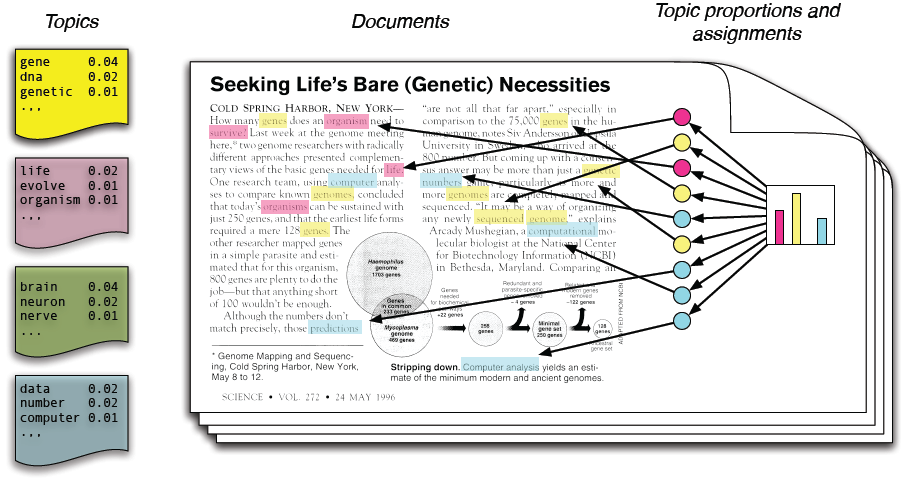
\includegraphics[scale=0.35]{img/gen}
\end{frame}

\section{PLSA, LDA and BigARTM}
\subsection*{Main Idea}

\begin{frame}
		\textcolor{red}{Probabilistic model}
		$$p(word | doc) = \sum_{topic} p(word | topic) p(topic|doc)$$
		
		\vspace{-0.3cm}
		\begin{itemize}
			\item The order of words in document is not matter (bag of words)
			\item Topic is not depends on doc ($p(word|doc, topic) = p(word| topic)$)
		\end{itemize}
		
		\vspace{-0.05cm}
		\textcolor{red}{Represent it as matrix decomposition} and solve this problem by MLE
		\begin{center}
			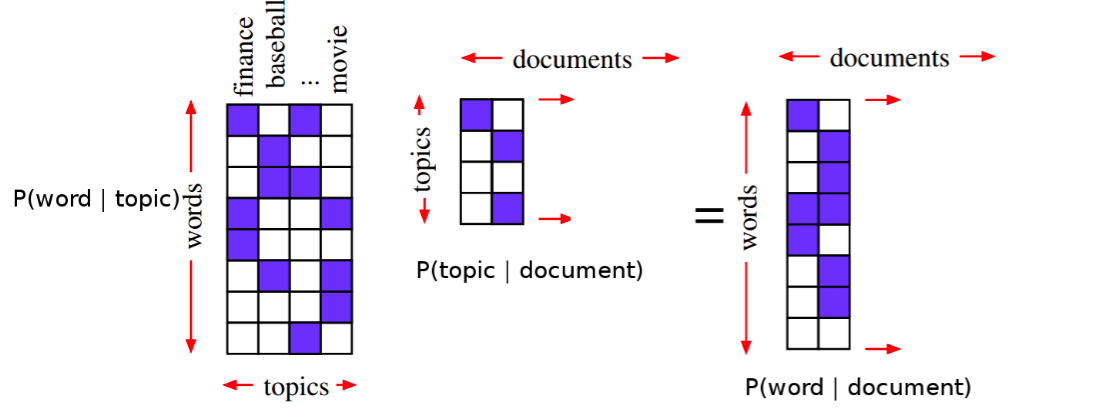
\includegraphics[scale=0.25]{img/mat_dec}
		\end{center} 
		
		\vspace{-0.5cm}
		\textcolor{red}{Regularization}
		\begin{itemize}
			\item LDA --  topics and documents generated from Dirichlet distribution
			\item BigARTM --  generalize LDA, many regularizes
		\end{itemize}
		
\end{frame}

\subsection*{Summary}
\begin{frame}
	\begin{itemize}
		\item[$+$] Good matrix approximation
		\item[$+$] A lot of implementations
		\item[$+$] There exist modification to take into account bigrams 
		\item[$-$] Solution is really depends on initial approximation
		\item[$-$] Poor model of documents
		\item[$-$] Difficult to parallelize
		\item[$-$] Computational difficult 
		\item[$-$] Control coefficient of regularizations is really hard task
	\end{itemize}
\end{frame}

\section*{Anchor Words}
\subsection*{Main Idea}
\begin{frame}
	\textcolor{red}{Let's assume} for each topic T there exist word $w$ that $p(w| t) \neq 0~if~t = T$
	
	\begin{center}
		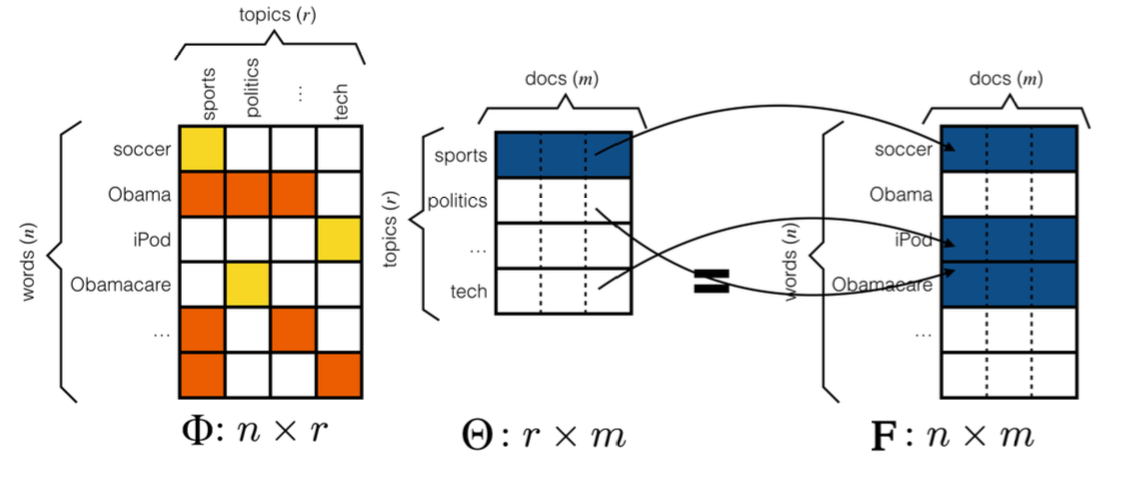
\includegraphics[scale=0.3]{img/anch_1}
	\end{center}
	
	Therefore F is a just a linear composition constructed  $\Theta$ rows, anchor rows.
	
	\begin{enumerate}
		\item How can we found rows in F which corresponds to anchor words?
		\item How can we reconstruct topic model $(\Phi, \Theta)$ given anchor words?
	\end{enumerate}
	
	
\end{frame}

\subsection*{More forml}
\begin{frame}
	\begin{itemize}
		\item Matrix F too noisy, let's use $FF^t$
		\item Size of $FF^t$ is $Words \times Words$ therefor reduce dimension
				$$FF^t_{words~\times~words} = H_{words \times k}$$ 
		\item Find almost convex hull in rows of H matrix $\{H_{anchor_1}, ..., H_{anchor_n}\}$
			\begin{center}
				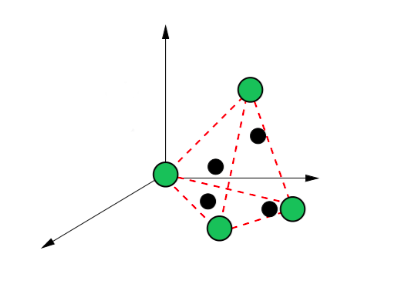
\includegraphics[scale=0.3]{img/hull}
			\end{center}
			
		\item Solve \textbf{undependent} convex optimization problems: find $c_i$ for each $t$
		$$ H_t \approx \sum_{i = 1, \dots, T} c_{ti} H_{anchor_i},~~c_{it} \geq 0,~~\sum_i c_{it} = 1, c_i = p(topic|word)$$
		\item Use Bayes rule to reconstruct $\Phi = (p(word|topic))_{W \times T}$
	\end{itemize}
\end{frame}

\subsection*{Summary}
\begin{frame}
	\begin{itemize}
		\item[$+$] No initial approximation
		\item[$+$] Very well parallelize out of box
		
		\item[$-$] Need to tune parameters
		\item[$-$] Can't take into account bigrams
		\item[$-$] Worst matrix decomposition
	\end{itemize}	
	
	\vspace{0.5cm}
	\textcolor{red}{Our goal was} propose modification witch \textbf{can take into account bigrams}.
	
	\vspace{0.5cm}
	\textcolor{red}{Why it is important?} 
	\begin{itemize}
		\item adding new information about word order in model
		\item better and lighter interpretability 
		\item simple solution -- does not work
	\end{itemize}
	 
\end{frame}

\section*{Bigramm Anchor Words}
\subsection*{Main Idea}

\begin{frame}
	There is one simple way:
		\begin{enumerate}
			\item precomputed bigrams
			\item we assume that  vector for bigram $w_iw_j$ = $H_{w_i}$ + $H_{w_j}$
			\item add vectors corresponds bigrams to set of points H (finding anchors)
			\begin{center}
					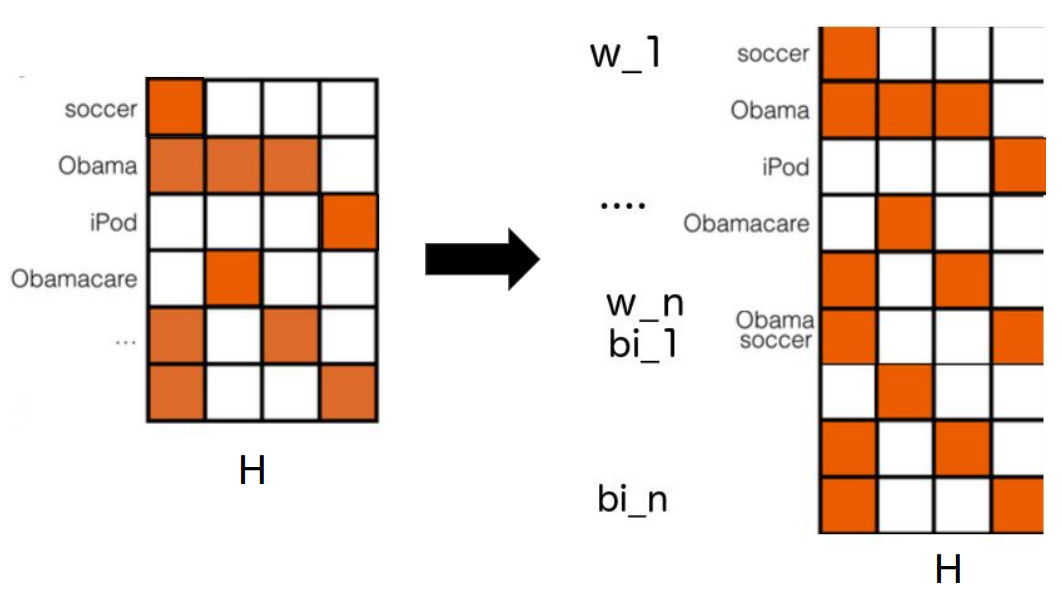
\includegraphics[scale=0.2]{img/h}
			\end{center}
			
			\vspace{-0.5cm}
			\item Find anchor words
			\item Recover topic mode
			\item Make some PLSA steps
		\end{enumerate}
		
		\vspace{0.1cm}
		\textcolor{red}{Bigrams} can be anchor words
		
		\textcolor{red}{Interpretations} good latent space in matrix H
		
\end{frame}

\section*{Evaluation}
\begin{frame}
	\begin{columns}[T] % align columns
		\begin{column}{.48\textwidth}
			\color{red}\rule{\linewidth}{4pt}
			
			Old anchors
			\begin{itemize}
				\item loss 
				\item cluster
				\item mixtur
				\item synaps
				\item theorem
				\item speech
				\item entropi
				\item filter
				\item competit
				\item gain
				\item markov
				\item identif
				\item algorithm 
			\end{itemize}
		\end{column}%
		\hfill%
		\begin{column}{.48\textwidth}
			\color{blue}\rule{\linewidth}{4pt}
			Our anchors
			
			\begin{itemize}
				\item mixtur
				\item \textcolor{red}{boltzmann\_machin}
				\item likelihood
				\item \textcolor{red}{markov\_chain}
				\item action
				\item \textcolor{red}{vector\_quantiz}
				\item network
				\item \textcolor{red}{robot\_arm}
				\item loss
				\item \textcolor{red}{tangent\_distanc}
				\item classifi
				\item \textcolor{red}{reinforc\_learn}
				\item speech
			\end{itemize}
			
			
		\end{column}%
	\end{columns}
	
\end{frame}

\section*{Metrics}
\begin{frame}
	Metrics:
	\begin{itemize}
		\item \textbf{Perplexity} is a mean $exp(-mean~likelihood)$
		\item \textbf{Coherence} is a mean Pointwise Mutual Information
		\item \textbf{Unique of kernels} is a mean Jaccard distance between most probable words in topic
	\end{itemize}
	
	{\small
		\begin{table}
			\centering
			\begin{tabular}{|l|l|l|l|l|l|l|l|l|l|}
				\hline
				\textbf{Collection} & \multicolumn{3}{l|}{\textit{\textbf{Banks Articles}}}    & \multicolumn{3}{l|}{\textit{\textbf{20 Newsgroups}}} & \multicolumn{3}{l|}{\textit{\textbf{~~~~~NIPS}}}    \\ \hline
				\textbf{Metric}   & \textit{$P_{test}$} & \textit{PMI}    & \textit{U}    & \textit{$P_{test}$}  & \textit{PMI}    & \textit{U}    & \textit{$P_{test}$} & \textit{PMI}    & \textit{U}    \\ \hline
				\texttt{PL}        & 2116                & 0.60          & 0.40          & 2155                 & 0.31          & 0.40          & 1635                & 0.21          & 0.32          \\ \hline
				\texttt{AW}        & 2330                & 0.63          & 0.53          & 2268                 & 0.38          & 0.41          & 1505                & 0.41          & 0.38          \\ \hline
				\texttt{BiAW}     & 2248                & 0.79          & 0.60          & 2183                 & 0.68          & 0.54          & 1500                &  0.50          &  0.41          \\ \hline
				\texttt{AW+PL}     & 2052                & 0.78          & 0.58          & 2053                 & 0.54          & 0.55          & 1434                & 0.52          & 0.46          \\ \hline
				\texttt{BiAW+PL}  & \textbf{1848}       & \textbf{0.87} & \textbf{0.63} & \textbf{2027}        & \textbf{0.78} & \textbf{0.64} & \textbf{1413}       & \textbf{0.58} & \textbf{0.49} \\ \hline
			\end{tabular}
		\end{table}}
\end{frame}

\section*{Bibliography}
\subsection*{Main papers}
\begin{frame}
	\begin{thebibliography}{10}
		\beamertemplatebookbibitems
		
		\item Arora, S., Ge, R., Moitra, A.: Learning topic models - going beyond svd. In:
		Foundations of Computer Science (FOCS), 2012 IEEE 53rd Annual Symposium
		on, IEEE (2012) 1–10
		\item Arora, S., Ge, R., Halpern, Y., Mimno, D., Moitra, A., Sontag, D., Wu, Y., Zhu,
		M.: A practical algorithm for topic modeling with provable guarantees. arXiv
		preprint arXiv:1212.4777 (2012)
		\item B, Dobrov, N, Loukachevitch: Forming the base of terminological phrases in the texts of the
		subject area (2003) 201–210
	\end{thebibliography}
\end{frame}

\end{document}

